% !TEX program = XeLaTeX
% !TEX encoding = UTF-8
\documentclass[UTF8,nofonts]{article}
%{ctexart}


%\setCJKmainfont[BoldFont=FandolSong-Bold.otf,ItalicFont=FandolKai-Regular.otf]{FandolSong-Regular.otf}
%\setCJKsansfont[BoldFont=FandolHei-Bold.otf]{FandolHei-Regular.otf}
%\setCJKmonofont{FandolFang-Regular.otf}
\usepackage[ngerman]{babel}
\usepackage[utf8]{inputenc}

\usepackage{url}
\usepackage{cancel}
\usepackage{xspace}
\usepackage{graphicx}
\usepackage{multicol}
\usepackage{multirow}
\usepackage{subfig}
\usepackage{amsmath}
\usepackage{amssymb}
\usepackage[a4paper, width=186mm, top=18mm, bottom=18mm, includeheadfoot]{geometry}
%\usepackage[a4paper, width=140mm, top=18mm, bottom=22mm, includeheadfoot]{geometry}
\usepackage{booktabs}
\usepackage{array}
\usepackage{verbatim}
\usepackage{caption}
\usepackage{natbib}
\usepackage{booktabs}
\usepackage{float}
\usepackage{pdflscape}
\usepackage{mathtools}
\usepackage[usenames, dvipsnames]{xcolor}
\usepackage{afterpage}
\usepackage{pgf}
\usepackage{tikz}
\usepackage{dirtree}
\usepackage[style=american]{csquotes}
\usepackage{amsfonts}
\usepackage{tikz}
\usepackage{tkz-graph}
\usetikzlibrary{arrows,decorations.pathmorphing,automata,positioning,backgrounds,fit,shapes.symbols,chains,intersections}

\newtheorem{definition}{Definition}[section]
\newtheorem{theorem}{Theorem}[section]
\newtheorem{lemma}{Lemma}
\newtheorem{proof}{Proof} [section]



\usepackage[toc, page, title, titletoc, header]{appendix}
\usepackage{marginnote}
\usepackage{tablefootnote}

%\renewcommand\appendixname{附\ 录}
%\renewcommand\appendixpagename{附\ 录}
%\renewcommand\appendixtocname{附\ 录}
\renewcommand\abstractname{Abstract}


\usepackage{perpage} %the perpage package
\MakePerPage{footnote} %the perpage package command

\usetikzlibrary{shapes.geometric}%
\usepackage{color}
%\usepackage[pages=some, placement=top]{background}
\usepackage{eso-pic}
\usepackage[final]{pdfpages}

%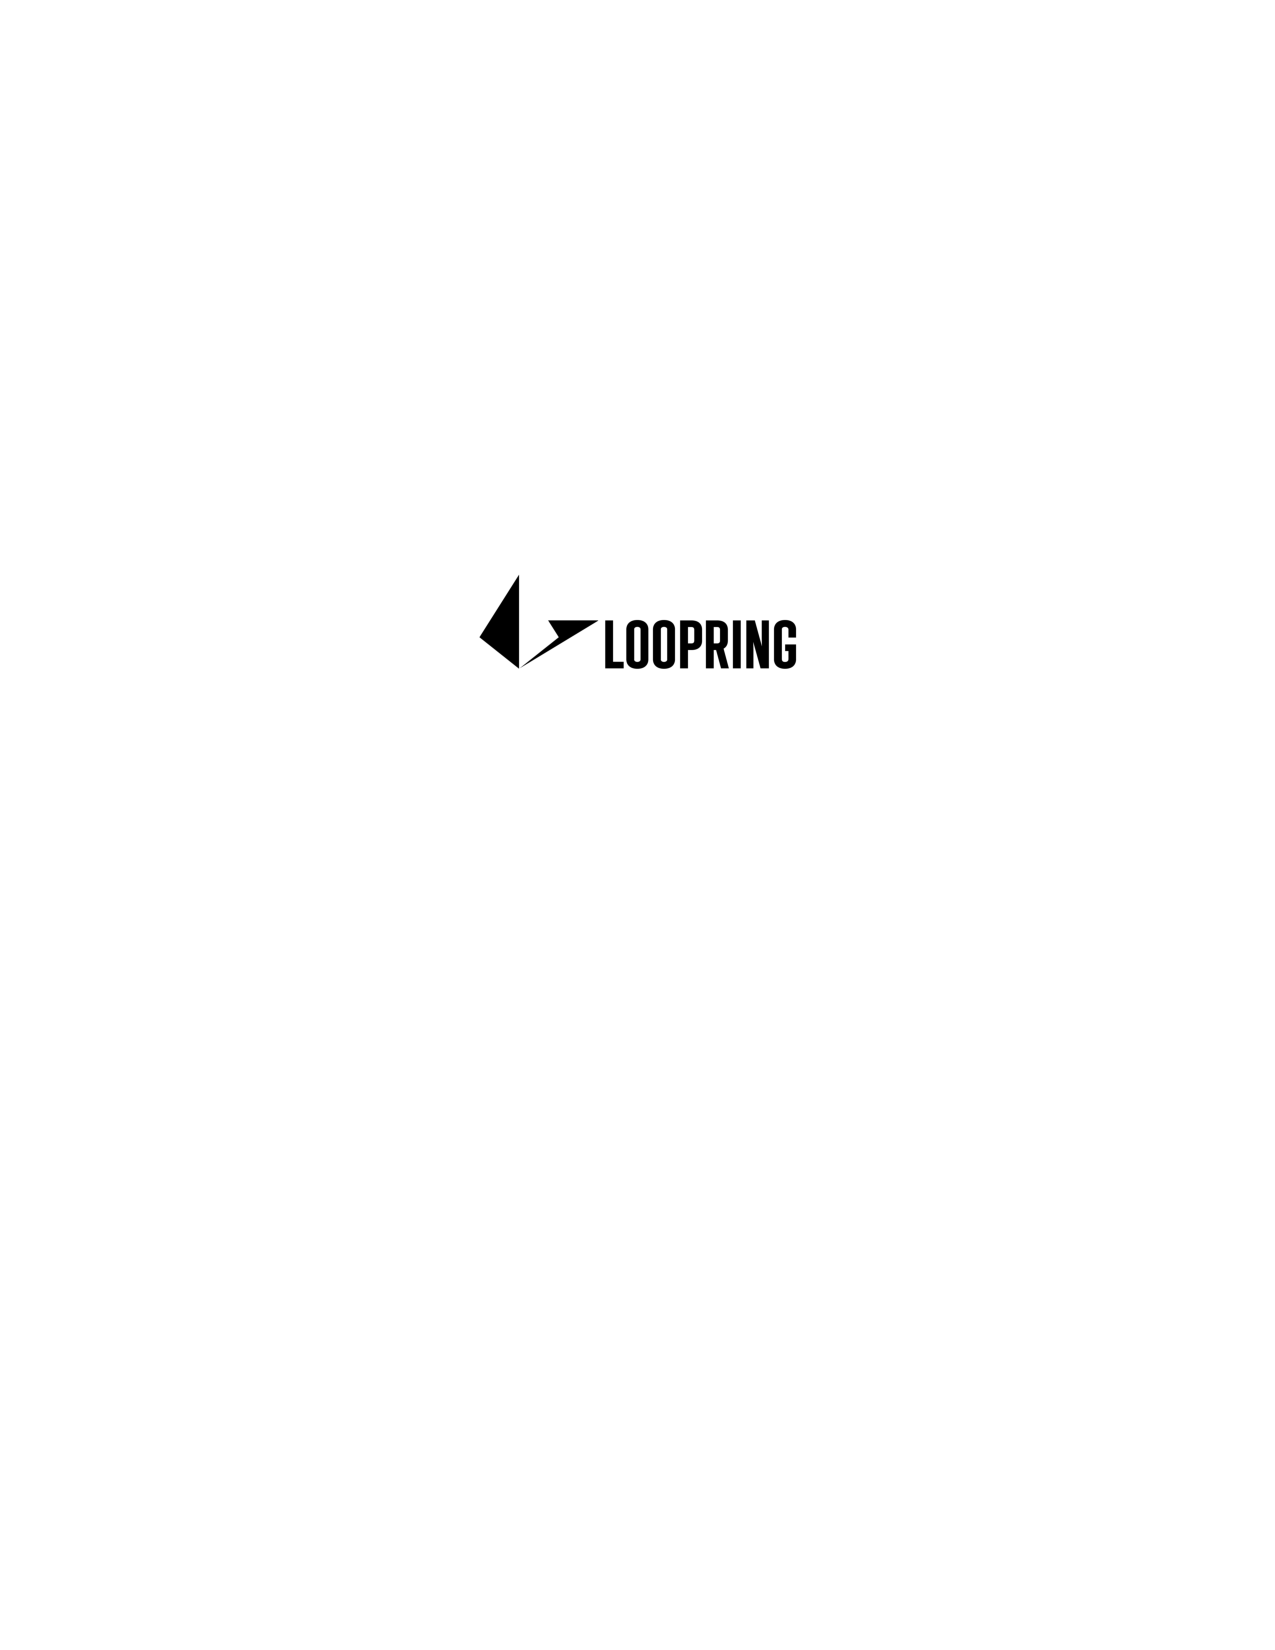
\includepdf[pages=1]{cover}
\hyphenpenalty=750

\title{\textbf{Loopring:}\\\textbf{Ein dezentrales Protokoll zum Tokenhandel}}
\author{
 Daniel Wang\\
  \texttt{daniel@loopring.org}\\
  \and
  	Jay Zhou\\
  	\texttt{jay@loopring.org}\\
  	\and
  	Alex Wang\\
  	\texttt{alex@loopring.org}\\
  	\and
  	Matthew Finestone\\
  	\texttt{matt.finestone@gmail.com}\\ 
  \\
  \texttt{https://loopring.org}
 }

%\makeatletter
%\def\CTEX@section@format{\Large\bfseries}
%\makeatother

\makeatletter
\newenvironment{tablehere}
 {\def\@captype{table}}
 {}

\newenvironment{figurehere}
 {\def\@captype{figure}}
 {}
\makeatother
%
%\newcommand\BackgroundPic{%
%\put(0, 0){%
%\parbox[b][\paperheight]{\paperwidth}{%
%\vfill
%\centering
%\includegraphics[width=\paperwidth, height=\paperheight, %
%%keepaspectratio]{images/background.jpg}%
%]{images/background.jpg}%
%\vfill
%}}}


\begin{document}
%\AddToShipoutPicture{\BackgroundPic}
\maketitle


\begin{abstract}
Loopring ist ein offenes Protokoll, um dezentrale Handelsplattformen zu vernetzen. Mittels öffentlicher Smart Contracts zur Ausführung des Tokenhandels werden Aufträge mehrerer Akteure gesammelt, ausgewertet und unabhängig der Blockchain durchgeführt. Es handelt sich um ein freies, erweiterbares Protokoll und dient als standardisierter Grundbaustein für dezentrale Applikationen (dApps), die den Handel von Tokens umfassen. Interoperable Standards ermöglichen einen vertrauensfreien, anonymen Handel. Eine wichtige Verbesserung gegenüber den derzeitigen dezentralen Austauschprotokollen ist die Möglichkeit, dass Aufträge mit anderen, unterschiedlichen Aufträgen gemischt werden können. Dadurch entfällt die Notwendigkeit von Zwei-Token-Handelspaaren und die Liquidität wird drastisch verbessert. Loopring verwendet eine einzigartige und solide Lösung, um ein Front-Running zu verhindern: der unfaire Versuch, Transaktionen schneller als der ursprüngliche Tauschanbieter in einen Block einzureichen. Loopring ist Blockchain-unabhängig und auf jede Blockchain mit Smart-Contract-Funktionalität anwendbar. Derzeit ist Loopring auf Ethereum \cite{buterin2017ethereum} \cite{wood2014ethereum} und Qtum \cite{dai2017smart} nutzbar und befindet sich für NEO \cite{atterlonn2018distributed} in der Entwicklung.
\end{abstract}



\begin{multicols}{2}
\section{Einleitung\label{sec:introduction}}
Mit der Verbreitung von Blockchain-basierten Vermögenswerten hat die Notwendigkeit, diese Güter untereinander auszutauschen, deutlich zugenommen. Da tausende neue Token zusätzlich zu traditionellen Vermögenswerte eingeführt werden, gibt es eine steigende Nachfrage. Unabhängig davon, ob Tokens zum spekulativen Handel oder für den Einsatz als Utility-Tokens auf Plattformen erworben werden, ist es essentiell für ein größeres Ökosystem, Krypto-Vermögenswerte untereinander austauschen zu können. Derzeit herrscht es eine wachsende Dynamik unter Vermögenswerten \cite{desotocapital}. Um diese zu ermöglichen und Kapital freizugeben, sind nicht nur Eigentumsrechte erforderlich, sondern auch die Möglichkeit, diese Vermögenswerte frei zu transferieren und zu transformieren.

Daher ist der Austausch von Tokens (Werten) ohne Zwischenhändler eine überzeugende Anwendung der Blockchain-Technologie. Dennoch haben sich Krypto-Enthusiasten bislang weitgehend für den Tokenhandel auf traditionellen, zentralisierten Handelsplattformen entschieden. Das Loopring-Protokoll wird benötigt, da - wie Bitcoin \cite{nakamoto2008bitcoin} bereits pflichtgemäß betonte - in Bezug auf elektronisches Geld \enquote{entscheidende Vorteile verloren gehen, wenn noch eine vertrauenswürdige dritte Partei benötigt wird, um doppelte Ausgaben zu vermeiden}. Von daher gehen die Hauptvorteile von dezentralen Vermögenswerten verloren, wenn sie über zentralisierte Handelsplattformen laufen müssen.

Der Handel dezentraler Tokens an zentralisierten Börsen ist auch aus philosophischer Sicht nicht nachvollziehbar, da die zugrundeliegende Idee, die dezentralisierte Projekte unterstützen, nicht zur Anwendung kommt. Es gibt auch zahlreiche praktische Risiken und Einschränkungen bei der Verwendung zentralisierter Vermittlungsstellen, die nachstehend beschrieben werden. Dezentralisierte Handelsplattformen (DEXs) \cite{schuh2015bitshares} \cite{bancor} \cite{kyber} haben versucht, diese Probleme zu lösen und in vielen Fällen ist es gelungen, Sicherheitsrisiken durch die Verwendung von Blockchains zur Einlagenumschichtung zu mindern. Da die Möglichkeiten dezentraler Handelsplattformen zu einer entscheidenden Infrastruktur für die neue Wirtschaft beitragen, gibt es erheblichen Spielraum für Leistungsverbesserungen. Loopring möchte Module für diese Infrastruktur mittels offenem Protokoll und der Erweiterbarkeit durch dApps bereitstellen.

\section{Aktuelle Handelsplattform-Landschaft\label{sec:current_exchange_landscape}}

\subsection{Unzulänglichkeiten von Zentralen Börsen}
Die drei Hauptrisiken zentraler Handelsplattformen sind; 1) Mangel an Sicherheit, 2) Mangel an Transparenz, und 3) Mangel an Liquidität.

\textbf{Ein Mangel an Sicherheit} ergibt sich daraus, dass Benutzer typischerweise die Kontrolle über ihre privaten Schlüssel (Mittel) an eine zentralisierte Einheit abgeben. Dies setzt die Benutzer der Gefahr aus, dass zentralisierte Austauschvorgänge böswilligen Hackern zum Opfer fallen. Die Sicherheits- und Hacking-Risiken \cite{coincheckhack}  \cite{mcmillan2014inside}, mit denen alle zentralisierten Börsen konfrontiert sind, sind allgemein bekannt, werden aber oft als Einsatz für den Token-Handel akzeptiert. Zentralisierte Plattformen sind nach wie vor Honeypots für Hackangriffe, da ihre Server über Millionen von Dollar an Benutzergeldern verfügen. Zusätzlich besteht immer die Möglichkeit, dass Angestellte einer Handelsplattform Fehler machen was zum Verlust der Gelder führt. Einfach gesagt, Benutzer haben nicht die Kontrolle über ihre eigenen Token, wenn sie an einer zentralisierten Handelsplattform hinterlegt werden.

\textbf{Ein Mangel an Transparenz} führt zu der Gefahr, dass unehrliche Handelsplattformen unfair agieren. Hier muss unterschieden werden da der Anwender nicht wirklich mit seinen eigenen Vermögenswerten handelt sondern sozusagen einen Schuldschein ausgestellt bekommt. Wenn die Token auf das Wallet der Handelsplattform gesendet werden, übernimmt die Handelsplattform die Verwahrung und bietet stattdessen einen Schuldschein an. Alle Tauschgeschäfte finden demnach zwischen den Schuldscheinen der Anwender statt. Um seine Token abheben zu können wird der Schuldschein eingelöst und man bekommt seine Token auf sein externes Wallet überwiesen. Während dieses Prozesses besteht ein Mangel an Transparenz und der Austausch kann zum Stillstand kommen, ihr Konto könnte eingefroren werden, die Handelsplattform könnte bankrott gehen, usw. Es ist auch möglich, dass sie Anwendervermögen für andere Zwecke verwenden, wie z. B. Ausleihen an Dritte. Ein Mangel an Transparenz kann Benutzer zusätzliche Kosten bescheren, ohne dass ein Totalverlust der Mittel eintritt, wie etwa höhere Handelsgebühren, Verzögerungen bei zu Spitzenzeiten, regulatorische Risiken und Aufträge die im Vordergrund stehen.

\textbf{Der Mangel an Liquidität.} Aus der Sicht der Betreiber einer Handelsplattform verhindert eine fragmentierte Liquidität den Einstieg neuer Börsen aufgrund von zwei Szenarien. Zum einen gewinnt die Handelsplattform mit der größten Anzahl von Handelspaaren, weil es für die Nutzer wünschenswert ist, alle ihre Geschäfte an einer Börse abzuwickeln. Zum anderen gewinnt die Handelsplattform mit dem größten Auftragsbuch aufgrund günstiger Bid-Ask Spannen für jedes Handelspaar. Dies erschwert den Wettbewerb durch Neulinge, da es für sie schwierig ist, eine initiale Liquidität aufzubauen. Infolgedessen haben viele Börsen einen hohen Marktanteil, trotz vieler Beschwerden von Benutzern und sogar größeren Hacking-Vorfällen. Es ist erwähnenswert, dass zentralisierte Börsen, welche schnell wachsen, zu einem immer größeren Angriffsziel für Hacker werden.

Aus der Sicht der Benutzer reduziert eine fragmentierte Liquidität die Benutzerfreundlichkeit erheblich. In einer zentralisierten Börse können Benutzer nur innerhalb der eigenen Liquiditätspools der Handelsplattform, gegen ihr eigenes Auftragsbuch und zwischen ihren unterstützten Token-Paaren handeln. Um ein Token für ein Token zu handeln, müssen Anwender an einer Handelsplattform handeln welche beide Token unterstützt oder sich an verschiedenen Handelsplattformen registrieren, wobei sie immer persönliche Informationen offenlegen. Benutzer müssen häufig vorläufige Transaktionen durchführen, in der Regel gegen BTC oder ETH, und dabei Bid-Ask-Spannen zahlen. Schließlich sind die Auftragsbücher möglicherweise nicht groß genug, um den Handel ohne einen niedrigeren initialen Preis abschließen zu können. Selbst wenn die Handelsplattform ein großes Volumen verarbeiten möchte, gibt es keine Garantie dafür, dass dieses Volumen und diese Liquidität nicht gefälscht sind \cite{fakevolume}.

Das Ergebnis sind getrennte Liquiditätsspeicher und ein fragmentiertes Ökosystem, das dem alten Finanzsystem ähnelt, mit bedeutendem Handelsvolumen, das an wenigen Handelsplattformen zentralisiert ist. Die globalen Liquiditätsversprechungen von Blockchains sind im zentralisierten Austausch nicht sinnvoll.

\subsection{Unzulänglichkeiten von dezentralisierten Handelsplattformen}
Dezentralisierte Handelsplattformen unterscheiden sich von zentralisierten Handelsplattformen zum Teil dadurch, dass Benutzer die Kontrolle über ihre privaten Schlüssel (Vermögenswerte) behalten indem sie Geschäfte direkt mit der zugrunde liegenden Blockchain abwickeln. Durch die Nutzung der Trustless-Technologie von Kryptowährungen selbst können viele der oben genannten Sicherheitsrisiken erfolgreich gemildert werden. Probleme bestehen jedoch hinsichtlich der Leistung und der strukturellen Einschränkungen.

Die Liquidität bleibt häufig ein Problem, da die Benutzer nach Gegenparteien in unterschiedlichen Liquiditätspools und -standards suchen müssen. Fragmentierte Liquiditätseffekte treten auf, wenn DEXs oder dApps insgesamt keine konsistenten Standards für die Interoperabilität verwenden und wenn Aufträge nicht über ein weites Netzwerk verteilt / verbreitet werden. Die Liquidität von Limit-Auftragsbüchern und insbesondere deren Ausfallsicherheit - wie schnell erfüllte Limit-Aufträgen neu generiert werden - können die optimalen Handelsstrategien erheblich beeinflussen \cite{limitorderliquidity}. Das Fehlen solcher Standards hat nicht nur zu einer verringerten Liquidität geführt, sondern auch zu einer Reihe von potenziell unsicheren proprietären Smart-Contracts. 

Da Transaktionen auf der Blockchain ausgeführt werden, erben DEXs außerdem die Beschränkungen der zugrunde liegenden Blockchain, nämlich: Skalierbarkeit, Verzögerungen bei der Ausführung (Mining) und kostspielige Änderungen an Aufträgen. Daher skalieren Blockchain-Auftragsbücher nicht besonders gut, da das Ausführen von Code auf der Blockchain Kosten (Gas) verursacht, wodurch mehrere Auftragsabbruch-Kadenzen unerschwinglich teuer werden.

Da die Auftragsbücher der Blockchain öffentlich sind, ist die Transaktion, um einen Kauf in Auftrag zugeben, für die Miner sichtbar, da die Transaktion abgearbeitet werden muss um danach in einem Auftragsbuch plaziert zu werden. Diese Verzögerung setzt den Benutzer dem Risiko aus, in Front zu laufen und den Preis oder die Ausführung gegen ihn zu bewegen.

\subsection{Hybride Lösungen}
Aus den obigen Gründen haben rein Blockchain-basierte Handelsplattformen Beschränkungen, die sie gegen zentralisierten Austauschen nicht wettbewerbsfähig machen. Es gibt einen Kompromiss zwischen der inhärenten Vertrauenswürdigkeit der Blockchain und der zentralisierten Austauschgeschwindigkeit und Auftragsflexibilität. Protokolle wie Loopring und 0x \cite{warren20170x} erweitern eine Lösung der On-Chain-Abwicklung mit Off-Chain-Order-Management. Diese Lösungen drehen sich um offene Smart Contracts, navigieren jedoch durch Skalierbarkeitsbeschränkungen indem sie mehrere Funktionen fernab der Blockchain ausführen und den Knoten Flexibilität bei der Erfüllung wichtiger Rollen für das Netzwerk geben. Die Nachteile bleiben jedoch auch für das Hybridmodell bestehen \cite{costofdecent}. Das Loopring-Protokoll schlägt in diesem Whitepaper sinnvolle Unterschiede in unserem Ansatz für eine hybride Lösung vor.

\section{Loopring Protokoll\label{sec:loopring_protocol}}
Loopring ist kein DEX, sondern ein modulares Protokoll zum Aufbau von DEXs auf mehreren Blockchains. Wir zerlegen die Bestandteile einer traditionellen Handelsplattform und bieten stattdessen eine Reihe von offenen Smart-Contracts und dezentralen Akteuren an. Zu den Rollen im Netzwerk gehören Wallets, Relais, Blockchains für Konsortien mit Liquiditätsteilung, Auftragsbuch-Browser, Ring-Miners und Vermögenswert-Tokenisierungsdienste. Bevor wir die einzelnen definieren, sollten wir zuerst die Loopring-Aufträge verstehen.

\subsection{Auftrags Ring\label{sec:order_ring}}
Loopring-Aufträge werden in einem sogenannten unidirektionalen Ordermodell (UDOM)\cite{coinport2014udom} ausgedrückt. UDOM drückt Aufträge als Token-Austausch-Anfragen aus, \verb|BetragS|/\verb|BetragB|, ( Betrag zu verkaufen/kaufen) statt Bids und Asks. Da jede Bestellung nur eine Austauschrate zwischen zwei Token ist, ist eine mächtige Eigenschaft des Protokolls das Mischen und Abgleichen mehrerer Bestellungen im Umlaufhandel. Durch den Einsatz von bis zu 16 Aufträgen anstelle eines einzelnen Handelspaars steigen die Liquidität und das Potenzial für eine Preisverbesserung dramatisch an.

\begin{center}
\begin{figurehere}
\centering
\tikzstyle{block} = [draw, fill=blue!20, rectangle, 
    minimum height=3em, minimum width=6em]
\tikzstyle{sum} = [draw, fill=blue!20, circle, node distance=1cm]
\tikzstyle{input} = [coordinate]
\tikzstyle{output} = [coordinate]
\tikzstyle{pinstyle} = [pin edge={to-,thin,black}]

\begin{tikzpicture}[
    auto, 
    node distance=2cm,
    >=latex',
    font=\bfseries\footnotesize\sffamily,
    order/.style={
		scale=0.7,
		rectangle,
		rounded corners,
		draw=black, 
		text centered,
%		text width=5cm,
		minimum height=12mm,
		fill=white
	},
	label/.style={
		scale=0.7
	}
  ]
    % We start by placing the blocks

  \node [order] (order2) 
 {%
 \begin{tabular}{l}
  \textbf{ORDER\#2}\\
  \textbf{owner: Y}\\
  \textbf{amountS: 9B}\\
  \textbf{amountB: 12C}
 \end{tabular}
 };
 
  \node [order, below of=order2, xshift=-3.5cm] (order1) 
 {%
 \begin{tabular}{l}
  \textbf{ORDER\#1}\\
  \textbf{owner: X}\\
  \textbf{amountS: 10000A}\\
  \textbf{amountB: 2B}
 \end{tabular}
 };
 
 
  \node [order, below of=order2, xshift=3.5cm] (order3) 
 {%
 \begin{tabular}{l}
  \textbf{ORDER\#3}\\
  \textbf{owner: Z}\\
  \textbf{amountS: 100C}\\
  \textbf{amountB: 160A}
 \end{tabular}
 };
 
 \draw [draw,->] (order1) -- node [label] {\textbf{7898A}} (order3);
 \draw [draw,->] (order2) -| node [label, xshift=-1.8cm] {\textbf{8B}} (order1);
 \draw [draw,->] (order3) |- node [label, xshift=1cm, yshift=0.24cm] {\textbf{98C}} (order2);

\end{tikzpicture}

\caption{A order-ring of 3 Orders}
\label{fig:ring}
\end{figurehere}
\end{center}


Die obige Abbildung zeigt einen Auftrags Ring mit drei Aufträgen. Jeder Auftrags Token der zum Verkauf steht (\verb|tokenS|), steht bei einem anderen Auftrag als Token zum Kauf (\verb|tokenB|). Es entsteht eine Schleife, die es jeder Bestellung erlaubt, ihre gewünschten Token zu tauschen, ohne eine gegenläufige Reihenfolge für ihr Paar zu benötigen. Herkömmliche Auftrags-Paar-Abwicklungen können natürlich noch ausgeführt werden, was im Wesentlichen ein Sonderfall eines Auftrags-Rings ist.

\begin{definition}[order-ring] $C_{0}$, $C_{1}$, $\cdots$, $C_{n-1}$ sind $n$ unterschiedliche Token, $O_{0\rightarrow 1}$, $\cdots$, $O_{i\rightarrow i\oplus 1}$, $\cdots$, $O_{n-1 \rightarrow 0}$ sind $n$ Aufträge. Diese Aufträge können einen Auftrags Ring formen:
$$O_{0\rightarrow 1} \rightarrow \cdots \rightarrow O_{i\rightarrow i\oplus 1} \rightarrow \cdots \rightarrow O_{n-1\rightarrow 0} \text{, }$$
wobei $n$ die Länge des Auftrags-Ringes ist, und $i\oplus 1 \equiv i+1 \mod n$.
\end{definition}

Ein Auftrags-Ring ist gültig, wenn alle Komponententransaktionen zu einem Wechselkurs ausgeführt werden können, der gleich oder besser ist als der ursprünglich implizit vom Benutzer festgelegte Kurs. Um die Gültigkeit des Auftrags-Rings zu überprüfen, müssen Smart-Contracts mit Loopring-Protokoll Auftrags-Ringe von Ring-Minern erhalten, wenn das Produkt der ursprünglichen Wechselkurse aller Orders gleich oder größer als 1 ist.

Nehmen wir an, Alice und Bob wollen ihr Token \verb|A| und \verb|B| tauschen. Alice hat 15 Token \verb|A| und sie möchte 4 Token \verb|B| dafür; Bob hat 10 Token \verb|B| und möchte 30 Token \verb|A| dafür.

Wer kauft und wer verkauft? Dies hängt nur von dem Token ab welcher als Referenz hergenommen wird. Wenn Token \verb|A| die Referenz ist, dann kauft Alice Token \verb|B| für den Preis von ${15 \over 4} = 3.75$\verb|A|, während Bob 10 Token \verb|B| für den Preis von ${30 \over 10} = 3.00$\verb|A| verkauft. Für den Fall das Token \verb|B| die Referenz ist, Alice verkauft 15 Token \verb|A| für den Preis von ${4\over 15}=0.26666667$\verb|B| und Bob kauft 10 Token \verb|A| für den Preis von ${10 \over 30}=0.33333334$\verb|B|. Deshalb ist der Käufer oder Verkäufer willkürlich.

Im ersten Fall ist Alice bereit einen höheren Preis ($3.75$\verb|A|) zu bezahlen als Bob ($3.00$\verb|A|) seine Token verkaufen würde, während im zweiten Fall Bob bereit ist einen höheren Preis ($0.33333334$\verb|B|) zu bezahlen als Alice ($0.26666667$\verb|B|) ihre Token verkaufen würde. Es ist klar, dass ein Handel möglich ist, wann immer der Käufer bereit ist, einen gleichen oder höheren Preis als den Preis des Verkäufers zu zahlen.

\begin{equation}
{{15\over 4} \over {30\over 10}} = {{10\over 30} \over {4\over 15}}={15 \over 4} \cdot {10 \over 30} = 1.25 > 1
\end{equation}

Damit ein Satz von $n$  Aufträgen ganz oder teilweise erfüllt werden kann, müssen wir also wissen, ob das Produkt eines jeden der Wechselkurse als Kaufaufträge zu einer Zahl größer oder gleich 1 führt. Wenn ja, können alle $n$  Aufträge entweder teilweise oder vollständig erfüllt werden. 

Wenn wir eine dritte Partei Charlie hinzufügen, so dass Alice $x_1$ Token \verb|A| geben und dafür $y_1$ Token \verb|B| erhalten möchte, Bob möchte $x_2$ Token \verb|B| geben und dafür $y_2$ Token \verb|C| erhalten möchte und Charlie möchte $x_3$ Token \verb|C| geben und dafür $y_3$ Token \verb|A| erhalten. Die erforderlichen Token sind vorhanden und der Handel ist möglich, wenn:

\begin{equation}
{{x1 \cdot x_2 \cdot x_3 \over y_1 \cdot y_2 \cdot y_3} \geq 1}
\end{equation}


Siehe Punkt \ref{anatomy} für detailliertere Informationen über Loopring Aufträge.



\section{Teilnehmer im Ökosystem\label{sec:ecosystem}}
Die folgenden Ökosystemteilnehmer stellen gemeinsam alle Funktionalitäten bereit, die ein zentralisierter Austausch bieten kann.

\begin{itemize}

\item \textbf{Wallets}: Ein allgemeiner Wallet-Service oder eine Schnittstelle, die Benutzern Zugriff auf ihre Token und eine Möglichkeit zum Senden von Aufträgen an das Loopring-Netzwerk bietet. Wallets werden durch das Teilen von Gebühren mit Ring-Minern angespornt Aufträge zu erstellen (siehe Abschnitt \ref{sec: token}). Mit der Überzeugung, dass die Zukunft des Handels innerhalb der sicheren Wallets einzelner Benutzers stattfinden wird, hat die Verbindung dieser Liquiditätspools durch unser Protokoll große Bedeutung.

\item \textbf{Konsortium liquiditätsteilende Blockchain/Relais-Netzwerke}: Ein Relais Netzwerk für Auftrags und Liquiditäts Teilung. Wenn einzelne Knoten die Loopring Relais Software verwenden, sind diese in der Lage einem bereits existierenden Netzwerk beizutreten und seine Liquidität über eine Konsortium Blockchain zu teilen. Die Konsortium Blockchain, die wir als erst Implementierung erstellten, hat nahezu Echtzeit-Auftragsteilung (1-2 Sekunden-Blöcke) und trimmt alte Historien, um ein schnelleres Herunterladen durch neue Knoten zu ermöglichen.

\item \textbf{Relais/Ring-Miner}: Relais sind Knoten welche Aufträge von Wallets oder Relais-Netzwerken erhalten, öffentliche Auftragsbücher und Auftrags Historien verwalten und optional Aufträge zu anderen Relais' übertragen (über irgendein beliebiges off-chain Medium). Ring-Minen ist ein Feature -- und keine Anforderung -- von Relais. Es ist rechenintensiv und erfolgt komplett fernab der Blockchain. Relais welche dieses Feature aktiviert haben werden \enquote{Ring-Miner} genannt, die Order-Ringe produzieren, indem sie unterschiedliche Aufträge zusammenfügen. Relays können frei wählen (1) wie sie sich untereinander verständigen, (2) wie sie ihre Auftragsbücher aufbauen und (3) wie sie Auftrags-Ringe abbauen (Mining-Algorithmen).

\item \textbf{Loopring Protokoll Smart Contracts (LPSC)}: Ein Set von öffentlich frei verfügbaren Smart Contracts welche Auftrags-Ringe von Ring-Minern überprüfen, Token im Namen der Anwender transferieren, den Ring-Minern und Wallets Anreize durch Gebühren geben und Events übertragen. Relays/Auftrags-Browser überwachen diese Ereignisse, um ihre Auftragsbücher und Handelshistorien aktuell zu halten. Siehe Anhang \ref{app:protocol_ethereum} für Details.

\item \textbf{Vermögenswert-Tokenisierungs-Service(VTS)}: Sie schlagen eine Brücke zwischen Vermögenswerten die nicht direkt über Loopring gehandelt werden können. Diese bestehen aus zentralisierten Diensten welche von vertrauenswürdigen Unternehmen oder Organisationen betrieben werden. Der Anwender deponiert Vermögenswerte (Real, Fiat, Token anderen Blockchains) und bekommt Token ausgestellt, die für eine Auszahlung eingelöst werden können. Loopring ist kein Blockchain übergreifendes Austauschprotokoll (bis eine geeignete Lösung existiert), jedoch ermöglicht VTS sowohl das Handeln von ERC20 Token \cite{ERC20} mit physikalischen Vermögenswerten als auch Vermögenswerte anderer Blockchains.

\end{itemize}


\section{Austauschprozess\label{sec:process}}



\begin{enumerate} 


\item \textbf{Protokollautorisierung}: In Abbildung \ref{fig:process} autorisiert, Inhaber \verb|Y|, der Token handeln möchte, autorisiert das LPSC \verb|BetragS| von Token \verb|B| zu verwalten, welche der Inhaber verkaufen möchte. Dies sperrt die Token des Inhabers nicht und ihm steht es frei die Token zu verschieben solange der Auftrag bearbeitet wird.

\item \textbf{Auftragserstellung}: Der aktuelle Preis und das Auftragsbuch für den Token \verb|B| gegen Token \verb|C| werden von Relais oder anderen Agenten, die mit dem Netzwerk verbunden sind,zur Verfügung gestellt, wie auch die Auftragsbuch-Browser. Inhaber \verb|Y| erstellt einen Auftrag (Limit Auftrag) spezifiziert \verb|BetragS| und \verb|BetragB| sowie andere Parameter durch jede mögliche Wallet Schnittstelle. Der Betrag an LRx kann dem Auftrag als Gebühr für Ring-Miner hinzugefügt werden; Höhere LRx Gebühren bedeuten eine höhere Chance früher von Ring-Minern bearbeitet zu werden. Der Hash des Auftrags wird durch den privaten Schlüssel von Inhaber \verb|Y| signiert.

\item \textbf{Auftragsverteilung}: Das Wallet überträgt den Auftrag und seine Signatur an ein oder mehrere Relais. Die/Das Relais aktualisieren/aktualisiert ihr Auftragsbuch. Das Protokoll schreibt nicht vor wie diese Auftragsbücher auszusehen haben, wie z.B. dass der erste Auftrag als erstes bearbeitet wird. Stattdessen haben Relais die Freiheit ihre eigenen Entscheidungen beim Aufbauen eines Auftragsbuches zu treffen.

\item \textbf{Liquidität teilen}: Relais verteilen den Auftrag über ein beliebiges Übertragungsmedium mit anderen Relais. Auch hier ist es flexibel wie Knoten miteinander interagieren. Um ein gewisses Maß an Netzwerkkonnektivität zu ermöglichen, gibt es ein integriertes Liquiditäts-Sharing-Relais-Netzwerk, das eine Konsortium-Blockchain verwendet. Wie im vorherigen Abschnitt erwähnt, ist dieses Relay-Netzwerk für Geschwindigkeit und Inklusivität optimiert.

\begin{center}
\begin{figurehere}
\centering
\tikzstyle{block} = [draw, fill=blue!20, rectangle, 
    minimum height=3em, minimum width=6em]
\tikzstyle{sum} = [draw, fill=blue!20, circle, node distance=1cm]
\tikzstyle{input} = [coordinate]
\tikzstyle{output} = [coordinate]
\tikzstyle{pinstyle} = [pin edge={to-,thin,black}]

\begin{tikzpicture}[
    auto, 
    scale=0.7,
    node distance=2cm,
    >=latex',
    font=\bfseries\footnotesize\sffamily,
    order/.style={
		rectangle,
		scale=0.7,
		rounded corners,
		draw=black, 
		text centered,
%		text width=5cm,
		minimum height=12mm,
		minimum width=30mm,
		fill=white
	},
	role/.style={
		circle,
		scale=0.7,
		draw=black, 
		text centered,
%		text width=5cm,
		minimum height=12mm,
		minimum width=12mm,
		fill=white
	},
	steps/.style={
		circle,
		scale=0.7,
		draw=black, 
		text centered,
%		text width=5cm,
%		minimum height=12mm,
%		minimum width=12mm,
		fill=black,
		text=white
	},
	account/.style={
		circle,
		scale=0.7,
		draw=black, 
		text centered,
%		text width=5cm,
		minimum height=16mm,
		minimum width=16mm,
		fill=white
	},
	label/.style={
	  scale=0.7
    }
  ]

 
 \node [role] (user1)  {user X};
 \node [role, below of=user1] (user2)  {user Y};
 \node [role, below of=user2] (user3)  {user Z};
 \node [role, below of=user3, fill=gray!20] (relay1)  {relay M};
 \node [role, below of=relay1, fill=gray!20] (relay2)  {relay N};

 
 \node [order, left of=user1, xshift=-1cm] (order1) 
 {%
 \begin{tabular}{l}
  \textbf{ORDER 1}\\
  \textbf{owner: X}\\
  \textbf{amountS: 10000 A}\\
  \textbf{amountB: 2 B}
 \end{tabular}
 };
 
 \draw [draw, ->]  (user1) -- (order1) [label]{};
 \draw [bend right,->] (order1) to node [auto, scale=0.7] {} (relay1);
 \draw [bend right,->] (order1) to node [auto, scale=0.7] {} (relay2);
% \draw [draw, ->]  (order1) |- (relay1) [label]{};
% \draw [draw, ->]  (order1) |- (relay2) [label]{};
 
 \node [order,left of=user2, xshift=-1.5cm] (order2) 
 {%
 \begin{tabular}{l}
  \textbf{ORDER 2}\\
  \textbf{owner: Y}\\
  \textbf{amountS: 9  B}\\
  \textbf{amountB: 12 C}
 \end{tabular}
 };
 \draw [draw, ->]  (user2) -- (order2) [label]{};
 \draw [bend right,->] (order2) to node [auto, scale=0.7] {} (relay1);
 \draw [bend right,->] (order2) to node [auto, scale=0.7] {} (relay2);
% \draw [draw, ->]  (order2) |- (relay1) [label]{};
% \draw [draw, ->]  (order2) |- (relay2) [label]{};
% 
\node [order, left of=user3, xshift=-2cm] (order3) 
 {%
 \begin{tabular}{l}
  \textbf{ORDER 3}\\
  \textbf{owner: Z}\\
  \textbf{amountS: 100 C}\\
  \textbf{amountB: 160 A}
 \end{tabular}
 };
 \draw [draw, ->]  (user3) -- (order3) [label]{};
 \draw [bend right,->] (order3) to node [auto, scale=0.7] {} (relay1);
 \draw [bend right,->] (order3) to node [auto, scale=0.7] {} (relay2);
% \draw [draw, ->]  (order3) |- (relay1) [label]{};
% \draw [draw, ->]  (order3) |- (relay2) [label]{};
 
% // The Ring
\node [order, 
yshift=-1.5cm,
xshift=-2.75cm,
below of=relay2,
fill=gray!10,
minimum width=4.2cm,
minimum height=5cm] (ring) {};


\node [order, dashed, below of=relay2,yshift=-0.2cm,xshift=-2.5cm] (order11) 
 {%
 \begin{tabular}{l}
  \textbf{ORDER 1}\\
  \textbf{owner: X}\\
  \textbf{amountS: 10000 A}\\
  \textbf{amountB: 2 B}
 \end{tabular}
 };
 \node [order, dashed,below of=order11,xshift=-0.25cm,yshift=0.7cm] (order21) 
 {%
 \begin{tabular}{l}
  \textbf{ORDER 2}\\
  \textbf{owner: Y}\\
  \textbf{amountS: 9  B}\\
  \textbf{amountB: 12 C}
 \end{tabular}
 };
\node [order, dashed,below of=order21,xshift=-0.25cm,yshift=0.7cm] (order31) 
 {%
 \begin{tabular}{l}
  \textbf{ORDER 3}\\
  \textbf{owner: Z}\\
  \textbf{amountS: 100 C}\\
  \textbf{amountB: 160 A}
 \end{tabular}
 };
 
 % // The blockchain
\node [
rectangle,
fill=gray!20, 
right of=user1,
yshift=-4.5cm,
xshift=0.1cm,
scale=0.7,
minimum width=3.2cm,
minimum height=15.6cm] (blockchain) {\parbox[b][15cm]{1.3cm}{blockchain}};
% blockchain accounts
  \node [account, right of=user1, xshift=1cm] (account1)  {accountX};
  \node [account, right of=user2, xshift=1cm] (account2)  {accountY};
  \node [account, right of=user3, xshift=1cm] (account3)  {accountZ};
  \node [account, right of=relay1, xshift=1cm] (account4)  {accountM};
  \node [account, right of=relay2, xshift=1cm] (account5)  {accountN};
  \node [account, double, below of=account5, yshift=-1.5cm] (psc)  {LPSC};
  
 \draw [draw, ->]  (user1) -- (account1) [label]{};
 \draw [draw, ->]  (user2) -- (account2) [label]{};
 \draw [draw, ->]  (user3) -- (account3) [label]{};
% \draw [draw, ->]  (relay1) -- (account4) [label]{};
% \draw [draw, ->]  (relay2) -- (account5) [label]{};
 \draw [draw, double, thick]  (relay1) to node [auto, scale=0.7] {share liquidity}  (relay2) [label]{};
% \draw [draw, ->]  (relay1) -- (ring) [label]{};
 \draw [draw, ->]  (relay2) to node [auto, scale=0.7, xshift=-1.8cm, yshift=0.3cm] {ring-mining}  (ring) [label]{};
 \draw [draw, ->]  (ring) to node [auto, scale=0.7] {submitRing} (psc) [label]{};
 
 \draw [bend left,->] (account1) to node [auto, scale=0.7] {\textbf{7898 A}} (account3);
 \draw [bend left,->] (account2) to node [auto, scale=0.7] {\textbf{8 B}} (account1);
 \draw [bend left,->] (account3) to node [auto, scale=0.7] {\textbf{98 C}} (account2);
 
 \draw [bend left,->, dashed] (account1) to node [auto, scale=0.7] {} (account5);
 \draw [bend left,->, dashed] (account2) to node [auto, scale=0.7] {} (account5);
 \draw [bend left,->, dashed] (account3) to node [auto, scale=0.7, xshift=.5cm] {\textbf{Fee}} (account5);
  
  
% \draw [draw,->] (order1) -- node [label] {\textbf{7898 A}} (order3);
% \draw [draw,->] (order2) -| node [label, xshift=-1.8cm] {\textbf{8 B}} (order1);
% \draw [draw,->] (order3) |- node [label, xshift=1cm, yshift=0.24cm] {\textbf{98 C}} (order2);

\node [steps, right of=user2, xshift=-0.6cm] () {1};
\node [steps, left of=user2, xshift=0.8cm] () {2};
\node [steps, left of=relay2, xshift=0.3cm, yshift=1cm] () {3};
\node [steps, left of=relay1, xshift=3.3cm, yshift=-1.6cm] () {4};
\node [steps, below of=relay2, xshift=-0.2cm, yshift=0.4cm] () {5};
\node [steps, right of=account3, xshift=-0.6cm] (step5) {6};

 \draw [bend right, ->]  (psc) to node [auto, scale=0.7, xshift=0.5cm] {settlement} (step5) [label]{};
 
\end{tikzpicture}

\caption{Loopring Exchange Process}
\label{fig:process}
\end{figurehere}
\end{center}

\item \textbf{Ring-Mining (Auftragsabgleich)}: Ring-Miner versuchen den Auftrag vollständig oder teilweise zu dem geforderten Preis oder besser zu erfüllen indem er mit mehreren anderen Aufträgen abgeglichen wird. Ring-Mining ist der Hauptgrund durch den das Protokoll hohe Liquidität zu jedem Paar bereitstellen kann. Wenn der ausgeführte Kurs besser ist als der von Benutzer Y angegebene Wert, wird die Marge unter allen Orders im Order-Ring geteilt. Als Belohnung wählt der Ring-Miner, ob er einen Teil der Marge (Margen-Split dem Benutzer die LRx zurückgeben) beansprucht oder einfach die LRx-Gebühr einbehält.

\item \textbf{Überprüfung \& Abrechnung}: Der Auftragsring wird von LPSC erhalten. Es führt mehrere Überprüfungen durch, um die von Ring-Minern gelieferten Daten zu verifizieren und stellt fest, ob der Bestellungsring ganz oder teilweise ausgeglichen werden kann (abhängig von der Füllrate von In-Ring-Bestellungen und Token in Benutzerportfolios). Wenn alle Überprüfungen erfolgreich sind, überträgt der Vertrag die Token automatisch an die Benutzer und zahlt gleichzeitig die Ring-Miner und Wallet-Gebühren. Wenn Inhabers \verb|Y| Saldo, nicht ausreicht, entschiden vom LPSC, wird dieser Auftrag als verkleinert angesehen: Ein verkleinerter Auftrag wird automatisch auf die initiale Größe hochgestuft wenn ausreichende Mittel zur Verfügung stehen, indem sie überwiesen werden, nicht wie ein Abbruch, welche nur in eine Richtung funktioniert und nicht rückgängig gemacht werden kann.

\end{enumerate}





%
%\end{multicols}
%
%\begin{center}
%\begin{figurehere}
%\includegraphics[height=8cm]{images/en_protocol.png}
%\caption{Loopring Trading Process}
%\label{fig: Loopringrotocol}
%\end{figurehere}
%\end{center}
%
%\begin{multicols}{2}

\section{Operative Flexibilität\label{sec:business_model}}
Es ist wichtig zu beachten, dass der freie Loopring Standard den Teilnehmern eine große Flexibilität bei der Bedienung ermöglicht. Akteuren steht es frei, neue Geschäftsmodelle zu implementieren und den Nutzern einen Mehrwert zu bieten, indem sie LRx-Gebühren für das Volumen oder andere Kennzahlen im Prozess verdienen (wenn sie dies wünschen). Das Ökosystem ist modular aufgebaut und soll die Teilnahme an einer Vielzahl von Anwendungen unterstützen.

\subsection{Auftragsbuch\label{sec:order_book}}
Relays können ihre Auftragsbücher auf verschiedene Arten gestalten, um die Bestellungen der Benutzer anzuzeigen und abzugleichen. Eine erste Implementierung unseres eigenen Auftragsbuches folgt einem OTC-Modell, bei dem Limit Aufträge nur auf Basis des Preises positioniert werden. Zeitstempel von Aufträgen haben also keine Auswirkungen auf das Auftragsbuch, jedoch steht es dem Relay frei, sein Auftragsbuch so zu gestalten, wie ein typisches Auftragsbuches einer zentralisierten Handelsplattform bei dem Zeitstempel ebenso berücksichtigt werden. Wenn ein Relay geneigt ist, diese Art von Auftragsbuch anzubieten, kann es ein Wallet integrieren und diese Wallet-Aufträge ausschließlich an dieses einzeln Relay schicken, welches dann in der Lage sein würde, die Aufträge zeitabhängig abzugleichen. Eine solche Konfiguration ist möglich. 

Während andere DEX-Protokolle zeitweise Ressourcen benötigen - anfängliche Token-Salden, um Taker-Aufträge zu platzieren - müssen Loopring-Relays nur nach zusammenpassenden Aufträgen suchen, um einen Handel zu vollenden. Sie können dies auch ohne initiale Token tun.

\subsection{Liquiditätsteilung\label{sec:liquidity_sharing}}
Relays können frei entscheiden, wie sie Liquidität (Aufträge) miteinander teilen. Unser Konsortium Blockchain ist nur eine Lösung um dies zu erreichen und dem Ökosystem steht es frei wie es vernetzt oder kommuniziert. Sie können sich nicht nur einer Blockchain eines Konsortiums anschließen, sondern auch eigene Regeln erstellen und verwalten und Regeln / Anreize erstellen, wenn sie es für richtig halten. Relays können auch alleine arbeiten, wie in der zeitsensitiven Wallet-Implementierung zu sehen ist. Natürlich gibt es klare Vorteile bei der Kommunikation mit anderen Relays bei der Verfolgung von Netzwerkeffekten, jedoch können verschiedene Business Modelle andere Verteilmöglichkeiten und Verteilen der Gebühren in Betracht ziehen.

\section{Protokoll Spezifikation\label{sec:protocol}}

\subsection{Anatomie eines Auftrags\label{anatomy}}
Ein Auftrag ist ein Datenpaket, das die Absicht des Handels des Benutzers beschreibt. Eine Loopring-Auftrag wird mithilfe des unidirektionalen Ordermodells (UDOM) wie folgt definiert:

\begin{verbatim}
  message Order {
    address protocol;
    address owner;
    address tokenS;
    address tokenB;
    uint256 amountS;
    uint256 amountB;
    unit256 lrcFee
    unit256 validSince; // Seconds since epoch
    unit256 validUntil; // Seconds since epoch
    uint8   marginSplitPercentage;  // [1-100]
    bool    buyNoMoreThanAmountB;
    uint256 walletId;
    // Dual-Authoring address
    address authAddr;
   	// v, r, s are parts of the signature
    uint8   v;       
    bytes32 r;
    bytes32 s;
    // Dual-Authoring private-key,
    // not used for calculating order's hash,
    // thus it is NOT signed.
    string  authKey;          
  }
\end{verbatim}

Um den Ursprung des Auftrags sicherzustellen, wird er gegen den Hash seiner Parameter signiert ohne \verb|authAddr|, mit dem privaten Schlüssel des Anwenders. Der \verb|authAddr| Parameter wird für das Signieren von Auftragsringen, dessen Teil dieser Auftrag ist um Front-Running zu vermeiden, verwendet. Weitere Informationen finden Sie in Abschnitt \ref{sec:dual_authoring}. Die Signatur wird durch \verb|v|, \verb|r|, und \verb|s| Felder dargestellt und wird zusammen mit den Auftragsparametern über das Netzwerk gesendet. Dies garantiert, dass die Bestellung während ihrer gesamten Lebensdauer unveränderbar bleibt. Auch wenn sich der Auftrag niemals ändert, kann das Protokoll seinen aktuellen Status basierend auf dem Saldo seiner Adresse zusammen mit anderen Variablen berechnen.

UDOM enthält keinen Preis (der von Natur aus eine Gleitkommazahl sein muss), sondern verwendet stattdessen den Begriff \verb|rate| oder $r$, welcher als \verb|amountS|/\verb|amountB| ausgedrückt wird. Der Preis ist keine Gleitkommazahl sondern ein Ausdruck, der nur mit anderen unsignierten Integer zahlen bei Bedarf evaluiert wird um alle Zwischenergebnisse als vorzeichenlose Ganzzahlen zu behalten und die Rechengenauigkeit zu erhöhen.

\subsubsection{Kaufbeträge}

Wenn ein Ring-Miner Aufträge abgleicht, besteht die Möglichkeit das eine bessere Rate ausführbar ist. Dies erlaubt es dem Anwender mehr \verb|tokenB| zu erhalten als \verb|amountB| spezifiziert war. Sollte jedoch \verb|buyNoMoreThanAmountB| auf \verb|True| gesetzt sein, dann stellt das Protokoll sicher dass der Anwendet nicht mehr als \verb|amountB| von \verb|tokenB| erhält. Somit bestimmt UDOM's \verb|buyNoMoreThantokenB| Parameter, wann ein Auftrag als vollständig erfüllt angesehen wird. \verb|buyNoMoreThantokenB| gilt als eine Obergrenze für entweder \verb|amountS| oder \verb|amountB| und erlaubt es dem Anwender, detailliertere Handelsabsichten auszudrücken als traditionelle Kauf- / Verkaufsaufträge.

Zum Beispiel: mit \verb|amountS| = 10 und \verb|amountB| = 2, wäre der Kurs $r$ = 10/2 = 5. Also möchte der der Anwender 5 \verb|tokenS| für jeden \verb|tokenB|. Der Ring-Miner gleicht ab und findet einen Anwender mit dem Kurs 4 welcher es dem Anwender erlaubt 2.5 \verb|tokenB| anstatt 2 zu erhalten. Sollte der Anwender jedoch nur 2 \verb|tokenB| wollen und hat den Parameter \verb|buyNoMoreThanAmountB| auf \verb|True| gesetzt, wird die Transaktion mit dem Kurs 4 und verkauft 4 \verb|tokenS| für jeden \verb|tokenB| und spart effektiv 2 \verb|tokenS|. Es muss jedoch beachtet werden das die Mining-Gebühren dabei nicht in Betracht gezogen werden (siehe Abschnitt \ref{sec:fee_model}).

Wenn wir Folgendes verwenden


\begin{verbatim}
	      Order(amountS,tokenS,
	            amountB,tokenB,
	            buyNoMoreThantokenB)
\end{verbatim}

um einen Auftrag vereinfacht darzustellen, dann können traditionelle Kauf-Verkauf-Modelle für die ETH / USD-Märkte an einer traditionellen Handelsplattform die erste und die dritte Order unten ausdrücken, aber nicht die anderen beiden:

\begin{enumerate}
	\item Verkaufe 10 ETH für 300 USD/ETH. Dieser Auftrag kann wie folgt dargestellt werden: \verb|Order(10, ETH, 3000, USD, False)|.
	\item Verkaufe ETH für 300 USD/ETH um 3000 USD zu erhalten. Dieser Auftrag kann wie folgt dargestellt werden: \verb|Order(10, ETH, 3000, USD, True)|.
	\item Kaufe 10 ETH um 300 USD/ETH, dieser Auftrag kann wie folgt dargestellt werden: \verb|Order(3000, USD, 10, ETH, True)|.
	\item Gebe 3000 USD aus um so viele ETH zu kaufen wie möglich für einen Preis von 300 USD/ETH, dieser Auftrag kann wie folgt dargestellt werden: \verb|Order(3000, USD, 10, ETH, False)|.
\end{enumerate}



\subsection{Ring Verifizierung\label{sec:ring_verification}}

Die Loopring Smart Contracts führen keine Wechselkurs- oder Mengenberechnungen durch, sondern müssen empfangen und überprüfen, was die Ring-Miner für diese Werte liefern. Diese Berechnungen werden aus zwei Gründen von Ring-Minern durchgeführt: (1) die Programmiersprache für Smart-Contracts, wie Solidity\cite{dannen2017introducing} auf Ethereum, unterstützt keine Gleitkomma-Berechnung, speziell $pow(x, 1/n)$ (Berechnung der n-ten Wurzel einer Gleitkommazahl) und (2) Es ist wünschenswert, dass die Berechnung außerhalb der Blockchain erfolgt, um die Blockchain-Berechnungskosten zu reduzieren.

\subsubsection{Sub-Ring Überprüfung\label{sec:sub_ring_check}}
Dieser Schritt verhindert, dass Arbitrageure die gesamte Marge in einem Auftragsring unfair realisieren, indem sie neue Aufträge implementieren. Sobald ein Ring-Miner einen gültigen Auftrags-Ring gefunden hat, könnte es verlockend sein, dem Auftrags-Ring weitere Aufträge hinzuzufügen, um die Marge des Benutzers vollständig zu absorbieren (Preisnachlässe). Wie unten in Abbildung \ref{fig:subring} dargestellt, zusammengezählt ergeben $x1$, $y1$, $x2$ und $y2$ das Produkt aller Kurse, genau 1, somit wird es keinen Preisnachlass geben.

\begin{center}
\begin{figurehere}
\centering
\tikzstyle{block} = [draw, fill=blue!20, rectangle, 
    minimum height=3em, minimum width=6em]
\tikzstyle{sum} = [draw, fill=blue!20, circle, node distance=1cm]
\tikzstyle{input} = [coordinate]
\tikzstyle{output} = [coordinate]
\tikzstyle{pinstyle} = [pin edge={to-,thin,black}]

\begin{tikzpicture}[
    auto, 
    node distance=2cm,
    >=latex',
    font=\bfseries\footnotesize\sffamily,
    order/.style={
		scale=0.7,
		rectangle,
		rounded corners,
		draw=black, 
		text centered,
%		text width=5cm,
		minimum height=12mm,
		fill=white
	},
	label/.style={
		scale=0.7
	}
  ]
    % We start by placing the blocks

  \node [order] (order2) 
 {%
 \begin{tabular}{l}
  \textbf{ORDER 2}\\
  \textbf{owner: Y}\\
  \textbf{amountS: 9B}\\
  \textbf{amountB: 12C}
 \end{tabular}
 };
 
  \node [order, below of=order2, xshift=-3.5cm] (order1) 
 {%
 \begin{tabular}{l}
  \textbf{ORDER 1}\\
  \textbf{owner: X}\\
  \textbf{amountS: 10000 A}\\
  \textbf{amountB: 2 B}
 \end{tabular}
 };
 
 
  \node [order, below of=order2, xshift=3.5cm] (order3) 
 {%
 \begin{tabular}{l}
  \textbf{ORDER 3}\\
  \textbf{owner: Z}\\
  \textbf{amountS: 100 C}\\
  \textbf{amountB: 160 A}
 \end{tabular}
 };
 
   \node [order, below of=order3, fill=gray!20] (order4) 
 {%
 \begin{tabular}{l}
  \textbf{ORDER 4}\\
  \textbf{owner: M}\\
  \textbf{amountS: x1 A}\\
  \textbf{amountB: y1 B}
 \end{tabular}
 };
 
 
  \node [order, below of=order1, fill=gray!20] (order5) 
 {%
 \begin{tabular}{l}
  \textbf{ORDER 5}\\
  \textbf{owner: addressM}\\
  \textbf{amountS: x2 C}\\
  \textbf{amountB: y2 A}
 \end{tabular}
 };
 
 \draw [draw,->] (order1) -- node [label, xshift=-2cm] {} (order5);
 \draw [draw,->] (order2) -| node [label, xshift=-1.6cm] {} (order1);
 \draw [draw,->] (order3) |- node [label, xshift=1cm] {} (order2);
 \draw [draw,->] (order4) -- node [label, xshift=1.8cm] {} (order3);
 \draw [draw,->] (order5) -- node [label, yshift=0.2cm] {} (order4);
  
\end{tikzpicture}

\caption{Ein Auftrags-ring mit Sub-Ring}
\label{fig:subring}
\end{figurehere}
\end{center}

Dies ist ein Null-Risiko, Null-Wert-Zusatz zum Netzwerk und wird als unfaires Verhalten des Ring-Miner angesehen. Um dies zu verhindern spezifiziert Loopring, dass eine gültige Schleife keine Sub-Ringe enthalten darf. Um dies zu überprüfen, stellt die LPSC sicher, dass ein Token nicht zweimal in einer Kauf- oder Verkaufsposition sein kann. Im obigen Diagramm können wir sehen, dass Token \verb|A| zweifach als Kauf und Verkauf verwendet wird. Dies wäre nicht erlaubt.

\subsubsection{Füllratenprüfung\label{sec:fill_rate_check}}

Die Wechselkursberechnungen im Auftrags-Ring werden von Ring-Miner aus den oben genannten Gründen vorgenommen. Es ist der LPSC, der sicherstellen muss, dass sie korrekt sind. Erstens überprüft es, ob die Kaufrate, die der Ring-Miner für jede Bestellung ausführen kann, gleich oder kleiner als die ursprüngliche Kaufrate ist, die vom Benutzer festgelegt wurde. Dies stellt sicher, dass der Benutzer mindestens den Wechselkurs erhält, den er verlangt oder besser. Sobald die Wechselkurse bestätigt sind, stellt der LPSC sicher, dass jede Bestellung im Auftrags-Ring den gleichen Preisnachlass teilt. Zum Beispiel, wenn der ermäßigte Kurs $\gamma$ ist, dann ist der Preis für jeden Auftrag: 

$r_{0\rightarrow 1} \cdot (1-\gamma)$, $r_{1\rightarrow 2} \cdot (1-\gamma)$, $r_{2 \rightarrow 0} \cdot (1-\gamma)$ und erfüllt:  
\begin{equation}
r_{0\rightarrow 1} \cdot (1-\gamma)\cdot r_{1\rightarrow 2} \cdot (1-\gamma) \cdot r_{2 \rightarrow 0} \cdot (1-\gamma) = 1
\end{equation}
deshalb:
\begin{equation}
\gamma = 1- \frac{1}{\sqrt[3]{r_{0\rightarrow 1} \cdot r_{1\rightarrow 2} \cdot r_{2\rightarrow 0}}}\text{.}
\end{equation}
Wenn die Transaktion $n$ Aufträge überschreitet, der \texttt{Diskont}: 
\begin{equation}
\gamma = 1- \frac{1}{\sqrt[n]{\prod_{i=0}^{n-1} r^i}} \text{,}
\end{equation}

wobei $r^i$ ist die Auftragsfluktuationsrate von $i$-ten Auftrag. Offensichtlich nur, wenn der Diskontsatz ist $\gamma \ge 0$, können diese Aufträge erfüllt werden; und der $i$-ten Auftrag ($O^i$)'s wirklicher Kurs ist $\hat{r^i} = r^i \cdot (1-\gamma)$, $\hat{r^i}\le r^i$.


\subsubsection{Erfüllungsverfolgung \& Abbruch}

Ein Benutzer kann einen Auftrag teilweise oder komplett abbrechen, indem er eine spezielle Transaktion an den LPSC sendet, die Informationen über den Auftrag und den abzubrechenden Betrag enthält. Der LPSC beachtet dies, speichert den abzubrechenden Betrag und sendet ein \verb|OrderCancelled| Event an das Netzwerk. Der LPSC verfolgt gefüllte und stornierte Beträge, indem sie ihre Werte mit dem Hash der Bestellung als Kennung speichert. Diese Daten sind offen einsehbar und \verb|OrderCancelled| / \verb|OrderFilled| Events werden gesendet wenn sie sich verändern. Das Verfolgen dieser Werte ist für den LPSC während des Auftragsring-Abrechnungsschritts kritisch.

LPSC unterstützt ebenso das Abbrechen aller Aufträge für ein Handelspaar mit dem \verb|OrdersCancelled| Event und das Abbrechen aller Aufträge für eine Adresse mit dem \verb|AllOrdersCancelled| Event.

\subsubsection{Auftragsskalierung\label{sec:order_scaling}}
Aufträge werden nach der Historie der erfüllten und stornierten Beträge und dem aktuellen Kontostand der Absender skaliert. Der Prozess findet den Auftrag mit dem kleinsten zu erfüllenden Betrag gemäß den obigen Merkmalen und verwendet ihn als Referenz für die Skalierung aller Transaktionen im Auftragsring.
Wenn der niedrigste Auftrag nach Wert gefunden wurde, kann das helfen das Füllvolumen für jede Bestellung zu ermitteln. Wenn zum Beispiel der $i$-te Auftrag der niedrigste wäre,  dann kann die Anzahl der von jeder Bestellung $\hat{s}$ verkauften Token und die Anzahl der von jeder Bestellung gekauften Token $\hat{b}$ berechnet werden:

\[
\begin{split}
&\hat{s}^{i}=\overline{s}_i\text{, } \hat{b}^{i}=\hat{s}^{i}/ \hat{r}^i\text{, }\text{;}\\
&\hat{s}^{i\oplus 1}=\hat{b}^i\text{, } \hat{b}^{i\oplus 1}=\hat{s}^{i\oplus 1}/ \hat{r}^{i\oplus 1}\text{;}\\
&\hat{s}^{i\oplus 2}=\hat{b}^{i\oplus 1}\text{, } \hat{b}^{i\oplus 2}=\hat{s}^{i\oplus 2}/ \hat{r}^{i\oplus 2}\text{;}\\
& ...
%\text{.}
\end{split}
\]
wobei $\overline{s}_i$ das Saldo ist, welches übrig bleibt nachdem die Aufträge teilweise erfüllt wurden.

Während der Implementierung können wir sicher annehmen, dass jeder Auftrag im Auftrags-Ring den niedrigsten Wert hat, und durchläuft dann den Auftrags-Ring höchstens zweimal um das Füllvolumen jeder Order zu berechnen.

Beispiel: Wenn der kleinste zu füllende Betrag im Vergleich zur ursprünglichen Reihenfolge 5\% ist, werden alle Transaktionen im Auftrags-Ring auf 5\% herunterskaliert. Sobald die Transaktionen abgeschlossen sind, sollte die Bestellung, die den geringsten noch zu füllenden Betrag aufweist, vollständig erfüllt werden.

\subsection{Ring Regelung\label{sec:settlement}}

Wenn der Auftrags-Ring alle vorherigen Prüfungen erfüllt hat, kann der Auftrags-Ring geschlossen und Transaktionen können durchgeführt werden. Dies bedeutet, dass alle $n$ Aufträge einen geschlossenen Auftrags-Ring bilden und verbunden sind wie in Abbildung 4:

\begin{center}
\begin{figurehere}
\centering
\begin{tikzpicture}[
circle/.style={
		scale=0.75,
		rounded corners,
		draw=black, 
		text centered,
		}
]

\def \n {6}
\def \m {4}
\def \radius {1.4cm}
\def \margin {12} % margin in angles, depends on the radius

\foreach \s in {1,...,\m}
{
  \node[draw, circle] at ({360/\n * (\s - 1)}:\radius) {$O^\s$};
  \draw[<-, >=latex] ({360/\n * (\s - 1)+\margin}:\radius) 
    arc ({360/\n * (\s - 1)+\margin}:{360/\n * (\s)-\margin}:\radius);
}

\node[draw, circle] at ({360/\n * 4}:\radius) {$O^5$};
  \draw[<-, dashed, >=latex] ({360/\n * 4+\margin}:\radius) 
    arc ({360/\n * 4+\margin}:{360/\n * (5)-\margin}:\radius);
    
\node[draw, circle] at ({360/\n * 5}:\radius) {$O^n$};
  \draw[<-, >=latex] ({360/\n * 5+\margin}:\radius) 
    arc ({360/\n * 5+\margin}:{360/\n * (6)-\margin}:\radius);


\end{tikzpicture}
\caption{Ring Regelung}
\label{fig:settlement}
\end{figurehere}
\end{center}

Um die Transaktion auszuführen verwendet der LPSC den \verb|TokenTransferDelegate| Smart-Contract. Die Einführung eines solchen Delegaten erleichtert die Aktualisierung des Protokoll-Smart-Contracts, da alle Aufträge nur diesen Delegaten anstelle verschiedener Versionen des Protokolls autorisieren müssen.

Für jeden Auftrag im Auftrags-Ring wird eine Zahlung von \verb|tokenS| für den nächsten oder vorhergehenden, abhängig von der Implementierung, Auftrag gemacht. Dann wird die Ring-Miner Gebühr abhängig vom Gebühren Modell, welches von dem Ring-Miner ausgewählt wurde bezahlt. Wurden alle Transaktionen ausgeführt wird ein \verb|RingMined| Event gesendet.

\subsubsection{Events\label{sec:events}}

Das Protokoll sendet Events, welche es Relays, Order-Browsern und anderen Teilnehmern erlauben Auftragsbuch-Aktualisierungen so effizient wie möglich zu erhalten. Die gesendeten Events sind:

\begin{itemize}
	\item \textbf{OrderCancelled}: Ein spezieller Auftrag wurde abgebrochen.
	\item \textbf{OrdersCancelled}: Alle Aufträge aller Handelspaare einer besitzenden Adresse wurden abgebrochen.
	\item \textbf{AllOrdersCancelled}: Alle Aufträge aller Handelspaare einer besitzenden Adresse wurden abgebrochen.
	\item \textbf{RingMined}: Ein Auftragsring wurde erfolgreich abgearbeitet. Dieses Event enthält Daten für jeden im Ring Token Transfer.
\end{itemize}


\section{LRx Token\label{sec:token}}
LRx ist unsere verallgemeinerte Tokennotation. LRC ist der Loopring Token auf Ethereum, LRQ auf Qtum und LRN auf NEO usw. Andere LRx-Typen werden in Zukunft eingeführt, wenn Loopring auf anderen öffentlichen Blockchains eingesetzt wird.

\subsection{Gebühren Modell\label{sec:fee_model}} 
Wenn ein Benutzer einen Auftrag erstellt, wird ein Betrag angegeben, der an die Ring-Miner als Gebühr bezahlt wird, in Verbindung mit einem Prozentsatz der Marge (\verb|marginSplitPercentage|) auf dem Auftrag, welche der Ring-Miner beanspruchen kann. Dies wird als Margensplit bezeichnet. Die Entscheidung welche (Gebühren- oder Margensplit), bleibt dem Ring-Miner überlassen.

Eine Darstellung des Margensplit: 

\begin{center}
\begin{figurehere}
\centering
\begin{tikzpicture}[
scale=1,
font=\bfseries\footnotesize\sffamily,
classical/.style={thick,<->,shorten >=2pt,shorten <=2pt,>=stealth},
oneway/.style={->,dashed,shorten >=2pt,shorten <=2pt,>=stealth}
]
    % Draw axes
    \draw [->,thick] (0,1) node (yaxis) [above] {$$}
        |- (6.2,0) node (xaxis) [right] {$$};
        
    \draw
  	(4,0) coordinate (A)
  	(4,1) coordinate (A2)
  	(4.8,-0.6) coordinate (B)
  	(4.8,1) coordinate (B2)
  	(6,-0.6) coordinate (C)
  	(6,1) coordinate (C2);
  	
  	\fill [draw=none, fill=gray!20] 
    (4.8, 0) rectangle (6, 1);
    
  	\fill [draw=none, fill=gray!10] 
    (0, -0.6) rectangle (4.8, 0);

	\draw[thick] (0, -0.6) -- (0, 0.6) node[below]{$$};
  	\draw[thick, thin] (A) -- (A2) node[below]{$$};
  	\draw[thick, thin] (B) -- (B2) node[below]{$$};
  	\draw[thick] (C) node[below, xshift=0.5cm]{$Total Buy Amount$} -- (C2) ;
  	
  	\draw[classical] (0, 0.5) -> (4, 0.5) node[below]{$$};
  	\draw[classical] (4, 0.75) -> (4.8, 0.75) node[below]{$$};
%  	\draw[classical] (4.8, 0.5) -> (6, 0.5) node[below]{$$};
  	\draw[classical] (4, 0.25) -> (6, 0.25) node[below]{$$};

  	
  	\draw[oneway] (2, 1.2) node[above]{$Order Original Buy Amount$} -- (2, 0.5);
  	\draw[oneway] (4.4, 2.2) node[above]{$Additional Buy Amount$} -- (4.4, 0.75);
  	\draw[oneway] (5.4, 1.6) node[above]{$Margin Split$} -- (5.4, 1);
  	\draw[oneway] (5, -1.2) node[below]{$Margin$} -- (5, 0.25);
  	\draw[oneway] (2.4, -1.2) node[below]{$Order Actual Buy Amount$} -- (2.4, -0.5);



\end{tikzpicture}
\caption{A 60\% Margin Split}
\label{fig:marginsplit}
\end{figurehere}
\end{center}

Wenn die Marge auf dem Auftrags-Ring zu klein ist, wählt ein Ring-Miner die LRx-Gebühr. Wenn die Marge im Gegensatz dazu so hoch ist, sodass der daraus resultierende Margensplit weit über die LRx-Gebühr hinausgeht, wählt ein Ring-Miner den Margensplit. Es gibt noch einen weiteren Vorbehalt: Wenn der Ring-Miner den Margensplit wählt, muss er dem Benutzer (Auftragserzeuger) eine Gebühr zahlen welche den LRx entspricht, die der Benutzer dem Ring-Miner als Gebühr gezahlt hätte. Dies erhöht den Schwellenwert für den Fall, in dem der Ring-Miner den Margensplit auf das Doppelte der LRx-Gebühr des Auftrags wählt. Dies macht die LRx-Gebühre attraktiver. Es ermöglicht den Ring-Minern, ein konstantes Einkommen auf Auftrags-Ringen mit niedriger Marge zu erhalten, um bei höheren Auftrags-Ringen weniger Erträge zu erhalten. Unser Gebühren Modell basiert auf der Erwartung, dass mit zunehmendem und reifendem Markt weniger Auftrags-Ringe mit hohen Margen auftreten und somit fixe LRx-Gebühren als Anreiz nötig sind. 

Am Ende steht folgender Graph:

\begin{center}
\begin{figurehere}
\centering
\begin{tikzpicture}[
font=\bfseries\footnotesize\sffamily,
oneway/.style={->,dashed,shorten >=2pt,shorten <=2pt,>=stealth},
scale=1]
    % Draw axes
    \draw [<->,thick] (0,2.7) node (yaxis) [above] {$y$}
        |- (5,0) node (xaxis) [right] {$x$};
        
    \draw
  	(1,1) coordinate (A)
  	(2,1) coordinate (B);
  	
  	
  	\draw[thick] (B) -- (3.7,2.7);
  	\draw[dotted] (B) -- (2,0) node[below] {$2f$};
  	\draw[dotted] (A) -- (1,0) node[below] {$f$};
  	\draw[thick,color=gray!70] (0,0) -- (2.7,2.7);
  	\draw[thick] (0,1) node[left] {$f$}--(B) node[     ]{$$};
 	\draw[oneway] (4,1) node[right]{$Expected Mining Income$} -- (3, 2);


\end{tikzpicture}
\caption{Loopring's Fee Model}
\label{fig:feemodel}
\end{figurehere}
\end{center}


wobei $f$ die LRx Gebühr ist, $x$ ist der Margensplit, $y$ ist das Mining Einkommen. $y=max(f, x-f)$ wie durch die durchgezogene Linie angezeigt; wenn die LRx Gebühr für den Auftrag $0$ ist, die Gleichung ist$y=max(0, x - 0)$ vereinfacht zu $y=x$ wie von der grauen Linie angezeigt wird.


Die Konsequenzen sind:
\begin{enumerate}
	\item Wenn der Margensplit 0 ist werden Ring-Miner die Flache LRx Gebührt wählen und sind immer noch motiviert.
	\item Wenn die LRx-Gebühr 0 ist, ergibt sich die graue Linie und das Einkommen basiert auf einem allgemeinen linearen Modell.
	\item Wenn das Margensplit-Einkommen größer als 2x ist (LRx-Gebühr), wählen die Ring-Miner den Margin-Split und zahlen LRx an den Nutzer.
\end{enumerate}

Es sollte angemerkt werden, dass, wenn die LRx Gebühr nicht Null ist, egal welche Option der Ring-Miner wählt, es immer eine Übertragung von LRx zwischen dem Ring-Miner und dem Absender des Auftrags geben wird. Entweder erhält der Ring-Miner die LRx-Gebühr oder zahlt die LRx-Gebühr an den Absender zurück, um den Margin-Split zu übernehmen.

Ring-Miner teilen einen bestimmten Prozentsatz der Gebühren mit Wallets. Wenn ein Benutzer einen Auftrag über ein Wallet abgibt und dieser erfüllt wird, wird das Wallet mit einem Teil der Gebühren oder der Margenaufteilung belohnt.Obwohl dies modular ist und einzigartige Geschäftsmodelle oder Implementierungen möglich sind, neigen wir dazu, dass Wallets etwa 20\% - 25\% der verdienten Gebühren erhalten. Wallets stellen ein Hauptziel für die Loopring-Protokollintegration dar, da sie die Benutzerbasis sind, aber wenig oder keine Einkommensquelle haben.

\subsection{Dezentralisierte Steuerung}
Das Loopring-Protokoll ist ein soziales Protokoll in dem Sinne, dass es auf Koordination zwischen den Mitgliedern angewiesen ist, um effektiv auf ein Ziel hin zu arbeiten. Dies ist den kryptoökonomischen Protokollen insgesamt nicht unähnlich, und in der Tat wird seine Nützlichkeit weitgehend durch die gleichen Mechanismen der Koordinationsprobleme \cite{vitalikgovernance}, des grimmigen Triggergleichgewichts und der beschränkten Rationalität geschützt. Zu diesem Zweck werden LRx-Token nicht nur zur Gebührenzahlung verwendet, sondern auch, um die finanziellen Anreize der verschiedenen Netzwerkteilnehmer in Einklang zu bringen. Eine solche Anpassung ist für die breite Verabschiedung eines Protokolls erforderlich und besonders wichtig für Austauschprotokolle, da der Erfolg weitgehend auf der Verbesserung der Liquidität in einem robusten dezentralen Ökosystem beruht.

LRx-Token werden verwendet, um Protokoll-Updates durch dezentrale Steuerung zu bewirken. Intelligente Vertragsaktualisierungen werden von Token-Inhabern geregelt, um Kontinuität und Sicherheit zu gewährleisten und die Risiken der Liquidität durch Inkompatibilität zu mindern. Angesichts der Tatsache, dass intelligente Verträge nach der Bereitstellung nicht mehr geändert werden können, besteht das Risiko, dass dApps oder Endbenutzer weiterhin mit veralteten Versionen interagieren und sich von aktualisierten Verträgen ausschließen. Die Aktualisierbarkeit ist entscheidend für den Erfolg des Protokolls, da es sich an die Marktanforderungen und die zugrunde liegenden Blockchains anpassen muss. Eine dezentrale Steuerung durch die LRx-Stakeholder ermöglicht Protokoll-Smart-Contract-Updates, ohne dApps oder Endbenutzer zu stören oder sich zu sehr auf die intelligente Vertragsabstraktion zu verlassen. Zunächst wird dies durch einen einfachen Multisignatur-Smart-Contract geschehen, um auf einen DAO-Typ-Mechanismus hinzuarbeiten.

\section{Betrugs- und Angriffsschutz}

\subsection{Front-Running-Prävention\label{sec:dual_authoring}}

In dezentralisierten Handelsplattformen bezeichnet man als Front-Running, wenn jemand versucht eine Handelsstrategie eines anderen Konten zu kopieren und zu verarbeiten bevor die ursprüngliche Transaktion welche sich noch im Pool befindet bearbeitet wird. Dies kann durch Angabe einer höheren Transaktionsgebühr (Gaspreis) erreicht werden. Das Hauptschema von Front-Running in Loopring (und jedes Protokoll mit Auftragsabgleichung) sind Auftrags-Filch: wenn ein Front-Runner einen oder mehrere Aufträge von einem ausstehenden Auftrags-Pool stiehlt und speziell im Fall von Loopring, wenn ein Front-Runner einen kompletten Auftrags-Ring einer ausstehenden Transaktion stiehlt.

Wenn eine submitRing Transaktion noch nicht bestätigt wurde und noch immer im ausstehenden Auftrags Pool ist. Diese kann von jedem einfach gefunden werden und \verb|minerAddress| kann mit der eigenen Adresse (\verb|filcherAddress|) ersetzt werden, danach können die Nutzdaten mit \verb|filcherAddress| erneut signiert werden. Der Fincher kann einen höheren Gas Preis setzen und eine neue Transaktion erstellen welche dann vor der ursprünglichen Transaktion von den Minern bearbeitet wird.

Frühere Lösungen für dieses Problem hatten wichtige Nachteile: sie erforderten mehr Transaktionen und somit kosten die Miner mehr Gas; benötigen doppelt so viele Blöcke um einen Auftrags-Ring abzuschließen. Unsere neue Lösung Dual-Authoring\cite{dualauthor}, umfasst den Mechanismus der Einrichtung von zwei Autorisierungsstufen für Aufträge - einen für die Abwicklung und einen für die Ring-Auftrags Abarbeitung..

Dual Authoring Prozess: 

\begin{enumerate}

	\item Für jeden Auftrag generiert die Wallet-Software ein zufälliges öffentliches / privates Schlüsselpaar und fügt das Schlüsselpaar in das JSON-Snippet des Auftrags ein. (Eine Alternative besteht darin, die vom öffentlichen Schlüssel abgeleitete Adresse anstelle des öffentlichen Schlüssels selbst zu verwenden, um die Bytegröße zu reduzieren. Wir verwenden \verb|authAddr| um eine solche Adresse darzustellen und \verb|authKey| anstatt \verb|authAddr|'s passenden privaten Schlüssel).

	\item Berechne den Auftrags Hash mit allen Feldern außer  \verb|r|, \verb|v|, \verb|s| und \verb|authKey|, signiere den Hash mit dem \verb|owner|'s privaten Schlüssel (nicht \verb|authKey|).

	\item Das Wallet sendet den Auftrag zusammen mit dem  \verb|authKey| zu den Relays um Ring-Mining zu ermöglichen. Ring-Miner überprüfen ob \verb|authKey| und \verb|authAddr| korrekt gepaart wurden und die Auftragssignatur mit der \verb|owner| Adresse übereinstimmt.

	\item Wenn ein Auftrags-Ring identifiziert wurde verwenden die Ring-Miner jedes Auftrags \verb|authKey| um den Ring Hash zu signieren, \verb|minerAddress| und alle anderen Mining Parameter. Enthält ein Auftrags-Ring $n$ Aufträge, so gibt es auch $n$ Signaturen von $n$ \verb|authKey|s. Wir nennen diese Signaturen \verb|authSignature|s. Der Ring-Miner muss möglicherweise auch den Hash des Rings zusammen mit allen Mining-Parametern unter Verwendung von\verb|minerAddress|'s privaten Schlüssels signieren.

	\item Der Ring-Miner ruft die submitRing Funktion mit allen Parametern und zusätzlich allen \verb|authSignature|s. \verb|authKey|s sind NICHT Teil der Blockchain Transaktion und bleiben deshalb für jeden außerhalb des Rings unbekannt.

	\item Das Loopring Protokoll wird nun alle \verb|authSignature| gegen die zugehörige \verb|authAddr| von jedem Auftrag verifizieren und den Ring ablehnen sollten \verb|authSignature|en fehlen oder ungültig sein..
 
\end{enumerate}

Das Ergebnis ist:

\begin{itemize}

	\item  Die Auftragssignatur (mit dem privaten Schlüssel \verb|owner|s Adresse) garantiert, dass der Auftrag inklusive der \verb|authAddr| nicht verändert werden kann.
	\item  Die Ring-Miner Signature (mit dem privaten Schlüssel \verb|minerAddress|), wenn mitgegeben, garantiert, dass niemand mit der gleichen Identität einen Auftrags-Ring abarbeiten kann.
	\item  Die \verb|authSignature|en versichern dass der gesammte Auftragsring nicht verändert werden kann, inklusive \verb|minerAddress| und Aufträge nicht gestohlen werden können.

\end{itemize}

Dual Authoring verhindert ring-Filch und order-Filch und stellt gleichzeitig sicher, dass die Abwicklung von Auftrags-Ringen in einer einzigen Transaktion durchgeführt werden kann. Darüber hinaus öffnet Dual Authoring Türen für Relays, um Aufträge auf zwei Arten zu teilen: nicht passende Freigabe und passende Freigabe. Standardmäßig arbeitet Loopring mit einem OTC-Modell und unterstützt nur Limit-Preis-Aufträge, d.h. die Zeitstempel der Aufträge werden ignoriert. Dies bedeutet, dass ein Front-Running eines Handels keine Auswirkungen auf den tatsächlichen Preis dieses Handels hat, sondern sich darauf auswirkt, ob er ausgeführt wird oder nicht. 

\section{Andere Angriffsszenarien}

\subsection{Sybil oder DOS Attacke}
Böswillige Benutzer -- handeln als sie selbst oder über gefälschte Identitäten -- könnte eine große Anzahl kleiner Aufträge senden, um Loopring-Knoten anzugreifen. Da wir es jedoch zulassen, dass Knoten Aufträge aufgrund eigener Kriterien ablehnen -- welche sie verstecken oder offenbaren können -- werden die meisten dieser Aufträge abgelehnt, wenn sie bei der Abstimmung keinen zufriedenstellenden Gewinn erzielen. Indem wir Relays befähigen, selbst zu entscheiden, wie sie Aufträge verwalten, sehen wir einen Angriff durch viele winzige Aufträge nicht als Bedrohung.

\subsection{Unzureichendes Guthaben}
Böswillige Benutzer können Aufträge bearbeiten und verteilen, deren Wert nicht Null ist, deren Adresse aber tatsächlich kein Guthaben hat. Knoten können überwachen und bemerken, dass der tatsächliche Saldo einiger Aufträge Null ist, sie aktualisieren diese Auftragszustände entsprechend und verwerfen Sie sie anschließend.
Knoten müssen Zeit investieren, um den Status eines Auftrags zu aktualisieren, können aber den Aufwand minimieren, indem sie beispielsweise Adressen auf die schwarze Liste setzen und zugehörige Bestellungen automatisch löschen.

\section{Conclusio}


Das Loopring-Protokoll ist eine grundlegende Schicht für den dezentralen Austausch. Dadurch hat es tiefgreifende Rückwirkungen auf den Austausch von Vermögenswerten und Werten. Geld, als eine Zwischenware, erleichtert oder ersetzt den Tauschhandel und löst das doppelte Zusammentreffen von Wunschproblemen\cite{unenumerated2006}, wobei zwei Kontrahenten das unterschiedliche Gut oder den Dienst des anderen begehren müssen. In ähnlicher Weise zielt das Loopring-Protokoll darauf ab, unsere Abhängigkeiten vom Zufall der Wünsche in Handelspaaren aufzuheben, indem Ring-Abgleich verwendet wird, um einen Handel leichter durchzuführen. Es ist bedeutsam wie die Gesellschaft und die Märkte Token, traditionelle Vermögenswerte und darüber hinaus austauschen. So wie dezentralisierte Kryptowährungen eine Bedrohung für die Kontrolle eines Landes über Geld darstellen, so ist ein kombinatorisches Protokoll, das Händler (Konsumenten / Produzenten) maßstabsgetreu zusammenbringen kann, eine theoretische Bedrohung für das Konzept des Geldes selbst.

Die Protokoll Vorteile umfassen:

\begin{itemize}
	\item Off-Chain-Auftragsverwaltung und On-Chain-Abwicklung bedeutet keine Leistungseinbußen für die Sicherheit.
	\item Höhere Liquidität durch Ring-Mining und Auftragsteilung.
	\item Dual Authoring löst das gefährliche Problem des Front Runnings, das heute von allen DEXs und ihren Benutzern bewältigt werden muss.
	\item Mit kostenlosen, öffentlichen Smart-Verträgen kann jede dApp das Protokoll erstellen oder mit diesem interagieren.
	\item Die Standardisierung unter den Operatoren ermöglicht Netzwerkeffekte und eine verbesserte Endbenutzererfahrung.
	\item Das Netzwerk wird mit Flexibilität in der Ausführung der Auftragsbücher und der Kommunikation aufrechterhalten.
	\item Geringere Eintrittsbarrieren bedeuten niedrigere Kosten für Knoten, die dem Netzwerk und den Endnutzern beitreten.
	\item Anonymes Handeln direkt vom privaten Wallet.
\end{itemize}

\section{Danksagungen}
Wir möchten unseren Mentoren, Beratern und den vielen Menschen in der Gemeinschaft, die so herzlich und großzügig mit ihrem Wissen waren, unseren Dank aussprechen. Insbesondere möchten wir Shuo Bai (von ChinaLedger); Professor Haibin Kan; Alex Cheng, Hongfei Da; Yin Cao; Xiaochuan Wu; Zhen Wang, Wei Yu, Nian Duan, Jun Xiao, Jiang Qian, Jiangxu Xiang, Yipeng Guo, Dahai Li, Kelvin Long, Huaxia Xia, Jun Ma und Encephalo Path für die Überprüfung des Projekts sowie das Feedback danken.


\bibliography{whitepaper}
\bibliographystyle{unsrt}


\end{multicols}


\begin{appendices}

\section{Loopring auf Ethereum\label{app:protocol_ethereum}}

\subsection{Smart Contracts}

\begin{center}
\begin{figurehere}
\centering
\begin{tikzpicture}
[node distance = 1cm, auto,font=\footnotesize,
% STYLES
every node/.style={node distance=3cm},
% The comment style is used to describe the characteristics of each force
comment/.style={rectangle, inner sep= 5pt, text width=4cm, node distance=0.25cm, font=\scriptsize\sffamily},
% The force style is used to draw the forces' name
force/.style={rectangle, draw, fill=black!10, inner sep=5pt, text width=4cm, text badly centered, minimum height=1.2cm, font=\bfseries\footnotesize\sffamily}] 

% Draw forces
\node [force] (impl) {LoopringProtocolImpl};
\node [force, dashed, above of=impl] (protocol_interface) {LoopringProtocol};
\node [force, left=1cm of impl] (nameregistry) {NameRegistry};
\node [force, right=1cm of impl] (tokenregistry) {TokenRegistry};
\node [force, below of=impl] (delegate) {TokenTransferDelegate};
\node [force, left=1cm of delegate] (multisig) {TransferableMultsig};

%%%%%%%%%%%%%%%
% Change data from here

% impl
\node [comment, below=0.25 of impl] (comment-impl) {- Validates order-rings\\
- Transfers tokens for settlement\\
- Emits events};

% nameregistry
\node [comment, below=0.25cm of nameregistry]{- Registers wallets and relays};

% protocol_interface
\node [comment, below=0.25 of protocol_interface](comment-interface) {- Defines interfaces and events};

% tokenregistry
\node [comment, below=0.25 of tokenregistry] {- Registers ERC20/ERC223 tokens};

% delegate
\node [comment, below=0.25 of delegate] {- Transfers tokens on behalf of users};

% PUBLIC POLICIES
\node [comment, text width=3cm, below=0.25 of multisig] {- Enables multisignature ownership};

%%%%%%%%%%%%%%%%

% Draw the links between forces
\path[->,thick] 
(comment-interface) edge (impl)
(nameregistry) edge (impl)
(tokenregistry) edge (impl)
(delegate) edge (comment-impl);

\end{tikzpicture} 
\caption{Smart Contracts}
\label{fig:smartcontracts}
\end{figurehere}
\end{center}

\subsection{Verteilung}

Die folgenden Smart Contracts wurden auf Ethereum Mainnet implementiert:
\begin{itemize}
\item LRC: \verb|0xEF68e7C694F40c8202821eDF525dE3782458639f|
\item TokenRegistry: \verb|0xa21c1f2AE7f721aE77b1204A4f0811c642638da9|
\item TokenTransferDelegate: \verb|0xc787aE8D6560FB77B82F42CED8eD39f94961e304|
\item NameRegistry: \verb|0x0f3Dce8560a6010DE119396af005552B7983b7e7|
\item LoopringProtocolImpl: \verb|0xc80BbAb86cED62CF795619A357581FaF0cB46511|
\item TransferableMultsig: \verb|0x7421ad9C880eDF007a122f119AD12dEd5f7C123B|
\end{itemize}

\end{appendices}
\end{document}
